\begin{tikzpicture}
    \node [anchor=west] (note) at (-1,3) {Curvature Note};
    \node [anchor=west] (water) at (-1,1) {First Bump};
    \begin{scope}[xshift=1.5cm]
        \node[anchor=south west,inner sep=0] (image) at (0,0) {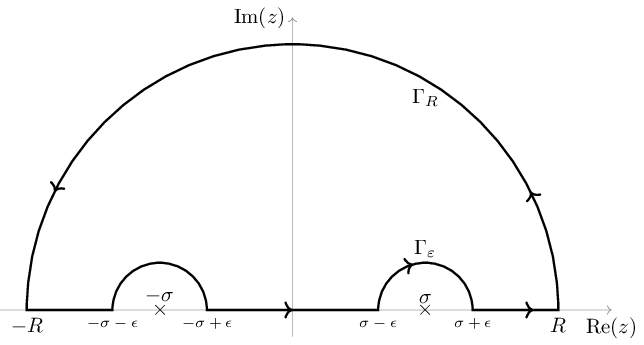
\includegraphics[width=0.7\textwidth]{../tikz/complex_integration_2.png}};
        \begin{scope}[x={(image.south east)},y={(image.north west)}]
            \draw[red,ultra thick,rounded corners] (0.48,0.80) rectangle (0.55,0.95);
            \draw [-latex, thick, red] (note) to[out=0, in=-120] (0.48,0.80);
            \draw [-stealth, line width=1pt, cyan] (water) -- ++(0.37,0.0);
        \end{scope}
    \end{scope}
\end{tikzpicture}%
